\section{If-statements}
\subsection{Uitleg}


\begin{frame}
\frametitle{Hoe kunnen we condities gebruiken in een programma?}

Allereerst\ldots Hoe gebruiken we condities in ons taalgebruik?

\vspace{15pt}
\visible<2->{``Als het regent, dan blijf ik binnen.''}

\visible<3->{``Als ik later groot ben, dan wordt ik een brandweerman.''}

\visible<4->{``Als ik die toets haal, dan ga ik over, of anders blijf ik zitten.''}

\vspace{15pt}
\visible<5->{In het algemeen:\\
``\textbf{Als} <<CONDITIE>>, \textbf{dan} <<ACTIE>>, \textbf{of anders} <<ACTIE>>''}

\end{frame}




\begin{frame}
\frametitle{Hoe kunnen we condities gebruiken in een programma?}

\visible<1->{``\textbf{Als} <<CONDITIE>>, \textbf{dan} <<ACTIE>>, \textbf{of anders} <<ACTIE>>. \textbf{Klaar}.''}

\vspace{3pt}
\visible<2->{``\textbf{If} <<CONDITION>>, \textbf{then} <<ACTION>>, \textbf{else} <<ACTION>>. \textbf{End}.''}

\vspace{15pt}
\visible<3->{
\begin{minipage}{0.43\textwidth}%
	\only<-4>{
		\begin{ticalc}[4.3cm]
			PROGRAM\:FIRST IF\\%
			\:If\,SOME\,CONDITION\\%
			\:Then\\%
			\:DO\,SOMETHING\\%
			\:Else\\%
			\:DO\,OTHER\,THING\\%
			\:End
		\end{ticalc}
	}\only<5->{
% 		\begin{figure}
% 			\hspace{-1.2cm}
% 		  	\centering
% 		    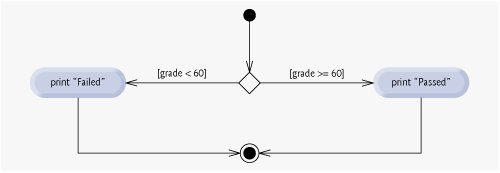
\includegraphics[width=1.2\textwidth]{../figures/IfDiagram.jpg}
% 		\end{figure}
		\begin{tikzpicture}[overlay,remember picture]
			\node [anchor=west,xshift=-0.9cm,yshift=0cm]
			{
			\begin{tikzonimage}[width=1.2\textwidth]{../figures/IfDiagram.jpg}
			\end{tikzonimage}
			};
		\end{tikzpicture}
	}
\end{minipage}%
~
\visible<4->{
\begin{minipage}{0.53\textwidth}%
	\begin{ticalc}[5.3cm]
		PROGRAM\:FIRST IF\\%
		\:If\,G\ge60\\%
		\:Then\\%
		\:Disp\,\qt PASSED.\qt\\%
		\:Else\\%
		\:Disp\,\qt FAILED.\qt\\%
		\:End
	\end{ticalc}
\end{minipage}%	
}
}

\vspace{5pt}
\visible<5->{Er ontstaan nu twee paden in het programma:\\}
\visible<6->{Slechts de statement(s) tussen \tifonttxt{Then} en \tifonttxt{Else} wordt uitgevoerd,
of de statement(s) tussen \tifonttxt{Else} en \tifonttxt{End}.}
\visible<7->{Daarna gaat het programma verder met statements die onder \tifonttxt{End} staan.}



% \begin{tikzpicture}[overlay,remember picture]
% 	\node[] (SE) at (current page.south east){ };
% 	\node [anchor=south east,xshift=0.05cm,yshift=1.4cm] at (SE)
% 	{
% 	\begin{tikzonimage}[height=#1]{../figures/IfDiagram.jpg}
% 	\end{tikzonimage}
% 	};
% \end{tikzpicture}

\end{frame}






\begin{frame}
\frametitle{Waar staat het op de GR?}

\visible<1-2,6->{\ticalcfig{\ticalcfigCircle{\ticalcfigCircleColThree}{0.615}}} % prgm
\visible<3>{\ticalcfig{}} % nothing
\visible<4-5>{\ticalcfig{\ticalcfigCircleSecond\ticalcfigCircle{\ticalcfigCircleColOne}{0.64}}} % test menu

\begin{itemize}
  \item<1-> Maak een nieuw programma: \inlineticalc{PROGRAM\:FIRSTIF}.
  \item<2-> Druk op \tiPRGM\,en kies \tifonttxt{If}.
  \item<3-> Type een letter.
  \item<4-> Druk op \tiTEST=\tiSecond\tiMATH\,en kies \tifonttxt{=}.
  \item<5-> Type \tifonttxt{0} gevolgd door \tiENTER.
  \item<6-> Druk op \tiPRGM\,en kies \tifonttxt{Then}, daarna \tiENTER.
  \item<7-> Druk op \tiPRGM\,en kies \tifonttxt{Else}, daarna \tiENTER.
  \item<8-> Druk op \tiPRGM\,en kies \tifonttxt{End}, daarna \tiENTER.
  \item<9-> Dit is de structuur van het \tifonttxt{if}-statement.
\end{itemize}


\begin{tikzpicture}[overlay,remember picture]
	\node[] (BL) at (current page.south east){ };
	\node [anchor=south east,xshift=0.195cm,yshift=0.6cm] at (BL)
	{%
	\only<1,3,5,9>{%
		\begin{ticalc}
			PROGRAM\:FIRSTIF\\%
			\:\only<1>{\tiCursor}\visible<3->{If\,A\only<3>{\tiCursor}\visible<5->{=0\\%
			\:\only<5>{\tiCursor}}}\visible<9->{Then\\%
			\:Else\\%
			\:End}\\%
			\visible<0>{.}
		\end{ticalc}
	}%
	\only<2>{%
		\begin{ticalc}
			\select{CTL}\,I/O\,EXEC \\
			\selectitem{1\+\:}If \\
			2\:Then \\
			3\:Else \\
			4\:For( \\
			5\:While \\
			6\:Repeat( \\
			7\arrowdown End
		\end{ticalc}
	}%
	\only<4>{%
		\begin{ticalc}
			\select{TEST}\,LOGIC \\
			\selectitem{1\+\:}= \\
			2\:\! \\
			3\:> \\
			4\:\ge \\
			5\:< \\
			6\:\le
		\end{ticalc}
	}%
	\only<6>{%
		\begin{ticalc}
			\select{CTL}\,I/O\,EXEC \\
			1\+\:If \\
			\selectitem{2\:}Then \\
			3\:Else \\
			4\:For( \\
			5\:While \\
			6\:Repeat( \\
			7\arrowdown End
		\end{ticalc}
	}%
	\only<7>{%
		\begin{ticalc}
			\select{CTL}\,I/O\,EXEC \\
			1\+\:If \\
			2\:Then \\
			\selectitem{3\:}Else \\
			4\:For( \\
			5\:While \\
			6\:Repeat( \\
			7\arrowdown End
		\end{ticalc}
	}%
	\only<8>{%
		\begin{ticalc}
			\select{CTL}\,I/O\,EXEC \\
			1\+\:If \\
			2\:Then \\
			3\:Else \\
			4\:For( \\
			5\:While \\
			6\:Repeat( \\
			\selectitem{7\arrowdown} End
		\end{ticalc}
	}%
	};
\end{tikzpicture}

\end{frame}



\subsection{Intermezzo: Invoegen/Insert}

\begin{frame}
\frametitle{Intermezzo: Invoegen/Insert}

\visible<3,5->{\ticalcfig{\ticalcfigCircleSecond\ticalcfigCircle{\ticalcfigCircleColThree}{0.8}}} % Ins
\visible<4>{\ticalcfig{\ticalcfigCircleSecond\ticalcfigCircle{\ticalcfigCircleColThree}{0.8}\ticalcfigCircleEnter}} % Ins + Enter
\visible<1,2>{\ticalcfig{}} % nothing

\begin{itemize}
  \item<2-> \lenitem{Plaats je cursor op \tifonttxt{Else}.}
  \item<3-> \lenitem{Druk op \tiINS=\tiSecond\tiDEL. Je cursor is nu verandert.}
  \item<4-> \lenitem{Druk op \tiENTER. Je hebt nu een regel \textit{boven} ingevoegd.}
  \item<5-> \lenitem{\tiINS=\tiSecond\tiDEL\,of de cursor bewegen be\"eindigd de insert-modus.}
\end{itemize}

\begin{tikzpicture}[overlay,remember picture]
	\node[] (BL) at (current page.south east){ };
	\node [anchor=south east,xshift=0.195cm,yshift=0.6cm] at (BL)
	{%
	\only<1>{%
		\begin{ticalc}
			PROGRAM\:FIRSTIF\\%
			\:If\,A=0\\%
			\:Then\\%
			\:Else\\%
			\:End\\%
			\visible<0>{.}
		\end{ticalc}
	}%
	\only<2>{%
		\begin{ticalc}
			PROGRAM\:FIRSTIF\\%
			\:If\,A=0\\%
			\:Then\\%
			\:\tiCursor lse\\%
			\:End\\%
			\visible<0>{.}
		\end{ticalc}
	}%
	\only<3>{%
		\begin{ticalc}
			PROGRAM\:FIRSTIF\\%
			\:If\,A=0\\%
			\:Then\\%
			\:\_lse\\%
			\:End\\%
			\visible<0>{.}
		\end{ticalc}
	}%
	\only<4>{%
		\begin{ticalc}
			PROGRAM\:FIRSTIF\\%
			\:If\,A=0\\%
			\:Then\\%
			\:\\%
			\:\_lse\\%
			\:End
		\end{ticalc}
	}%
	\only<5->{%
		\begin{ticalc}
			PROGRAM\:FIRSTIF\\%
			\:If\,A=0\\%
			\:Then\\%
			\:\\%
			\:Else\\%
			\:End
		\end{ticalc}
	}%
	};
\end{tikzpicture}


\end{frame}

\subsection{Zelf Oefenen}


\begin{frame}
\frametitle{Oefening!}

Schrijf het volgende \tifonttxt{Prgm} op je GR (bedenk zelf een leuke naam):

\begin{itemize}
  \item Vraag de gebruiker om een cijfer, $G$.
  \item Daarna: \textbf{Als} <<Cijfer 6 of hoger>>, \textbf{dan} <<Weergeef \tifonttxt{OK}>>, \textbf{of anders} <<Weergeef \tifonttxt{FAIL}>>.
  \item Breid dit programma uit zodat een cijfer boven 8 \tifonttxt{GOOD} en boven 9.5 \tifonttxt{PERFECT} zegt.
  \item Controleer of $G$ wel een cijfer is! (Waar moet een cijfer aan voldoen?) Geef een foutmelding indien $G$ geen cijfer kan zijn.
  		\footnotesize{Tip: Je kunt gebruik maken van \inlineticalc{Stop} uit het \tiPRGM\inlineticalc{CTL} menu.}
\end{itemize}

\visible<2->{Merk op dat we het programma in stappen schreven, dit is volgens het `Scrum' programmeer-paradigma:
``Maak eerst een werkend programma, voeg daarna nieuwe features toe!''}

\end{frame}


\begin{frame}
\frametitle{Oefening! \tifonttxt{\>} Antwoord}

\begin{minipage}{0.4\textwidth}
\begin{ticalc}
	PROGRAM\:GRADER\\%
	\:Input\,\qt GRADE?\,\qt\comma G\\%
	\:If\,G<1\,or\,G>10\\%
	\:Then\\%
	\:Disp\,\qt INVALID GRADE\qt\\%
	\:Stop\\%
	\:End\\%
	\:If\,G\ge6
	\:Then\\% >=6
	\:If\,G\ge8
	\:Then\\% >=8
	\:If\,G\ge9.5
	\:Then\\% >=9.5
	\:Disp\,\qt PERFECT\qt\\%
	\:Else\\% >=8 and <9.5
	\:Disp\,\qt GOOD\qt\\%
	\:End\\%
	\:Else\\% >=6 and <8
	\:Disp\,\qt OK\qt\\%
	\:End\\%
	\:Else\\% <6
	\:Disp\,\qt FAIL\qt\\%
	\:End
\end{ticalc}
\end{minipage}
\begin{minipage}{0.58\textwidth}
Dit is een mogelijk antwoord.
Uiteraard zijn er meerdere mogelijkheden. Zolang het resultaat maar hetzelfde is!

\vspace{1cm}
Merk op dat ik hier \inlineticalc{Input} gebruik, i.p.v. \inlineticalc{Prompt}.
Het werkt hetzelfde, maar heeft als eerste argument een string, hier: ``\tifonttxt{Grade?\,}''.
\end{minipage}

\end{frame}







